\documentclass[a0,portrait]{a0poster}

\usepackage[margin=3cm]{geometry}
\usepackage{multicol}
\columnsep=100pt
\columnseprule=1pt
\usepackage[svgnames]{xcolor}
\usepackage{palatino}
\usepackage{amsmath}
\usepackage{graphicx}
\usepackage{booktabs}
\usepackage[labelfont=bf]{caption}
\usepackage{amsfonts, amsmath, amsthm, amssymb}
\usepackage{wrapfig}
\usepackage{caption}
\usepackage[caption=false]{subfig}
\usepackage{textcomp}
\usepackage{bm}

\usepackage{pifont}
\usepackage{xcolor}
\definecolor{myblue}{RGB}{50,150,90}

\newcommand{\bi}{\item[\color{myblue}\ding{108}]} 

\begin{document}

\begin{minipage}[b]{0.3\linewidth}
\centering

\includegraphics[width=25cm]{../fig/umk.png}
\end{minipage}\hspace*{4cm}
\begin{minipage}[b]{0.3\linewidth}
\centering

\includegraphics[width=23cm]{../fig/mpip.png}
\end{minipage}\hspace*{3cm}
\begin{minipage}[b]{0.3\linewidth}
\centering

\includegraphics[width=16cm]{../fig/helmut.jpg}
\end{minipage}

\vspace{1cm}

\begin{minipage}[b]{\linewidth}
\veryHuge\centering\color{myblue} 
\begin{minipage}[b]{\linewidth}
\textbf{Enhanced Sampling Method for Ligand Unbinding}
  \end{minipage}
\end{minipage}
\color{Black}\\[1cm]
\begin{minipage}[b]{\linewidth}
  \huge \textbf{Jakub Rydzewski$^1$}, Omar Valsson$^2$, and Helmut
  Grubm\"{u}ller$^3$\\[1cm]
\large $^1$ Institute of Physics, Nicolaus Copernicus University,
  Grudziadzka 5, 87-100 Torun, Poland\\
\large $^2$ Max Planck Institute for Polymer Research, Ackermannweg 10,
  D-55128 Mainz, Germany\\
\large $^3$ Max Planck Institute for Biophysical Chemistry, Am Fassberg 11,
  37077 Göttingen, Germany\\
\end{minipage}

\vspace{1cm}

\begin{multicols}{2}
\large
\section*{\huge\centering\color{myblue}How to Find an Exit Tunnel?}
\vspace*{1cm}
\begin{minipage}[b]{\linewidth}
  \centering
  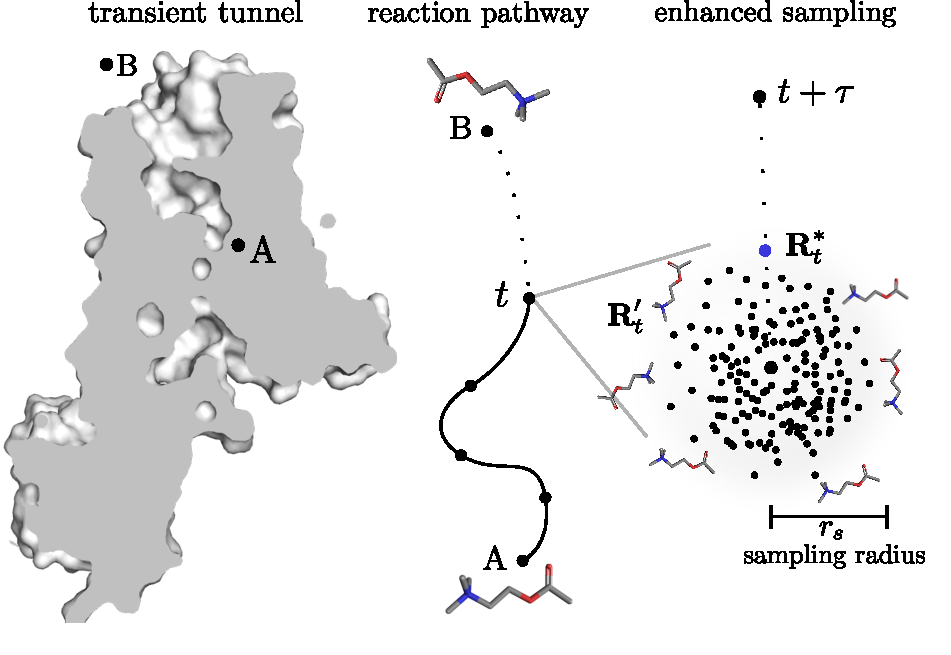
\includegraphics[width=36cm]{../fig/fig0a.pdf}
\end{minipage}

\begin{minipage}[b]{0.5\linewidth}
  \centering
  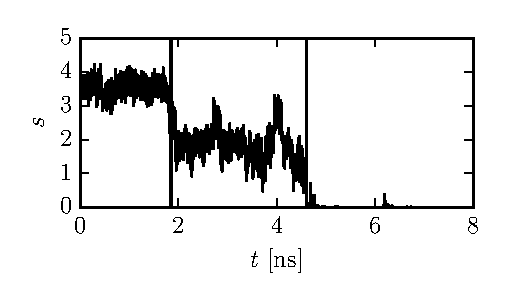
\includegraphics[width=20cm]{../fig/fig2.pdf}
\end{minipage}
\hspace{1cm}
\begin{minipage}[b]{0.4\linewidth}
  \begin{itemize}
    \bi Enhanced sampling and non-convex optimization;
    \bi Biasing toward the minimum of the loss function;
    \bi Loss function describes interactions in a ligand-protein system;
  \end{itemize}
  \vspace*{1cm}
\end{minipage}

\section*{\huge\centering\color{myblue}Slow-Onset Inhibitor Unbinding}
\vspace*{1cm}
\begin{minipage}[b]{\linewidth}
  \centering
  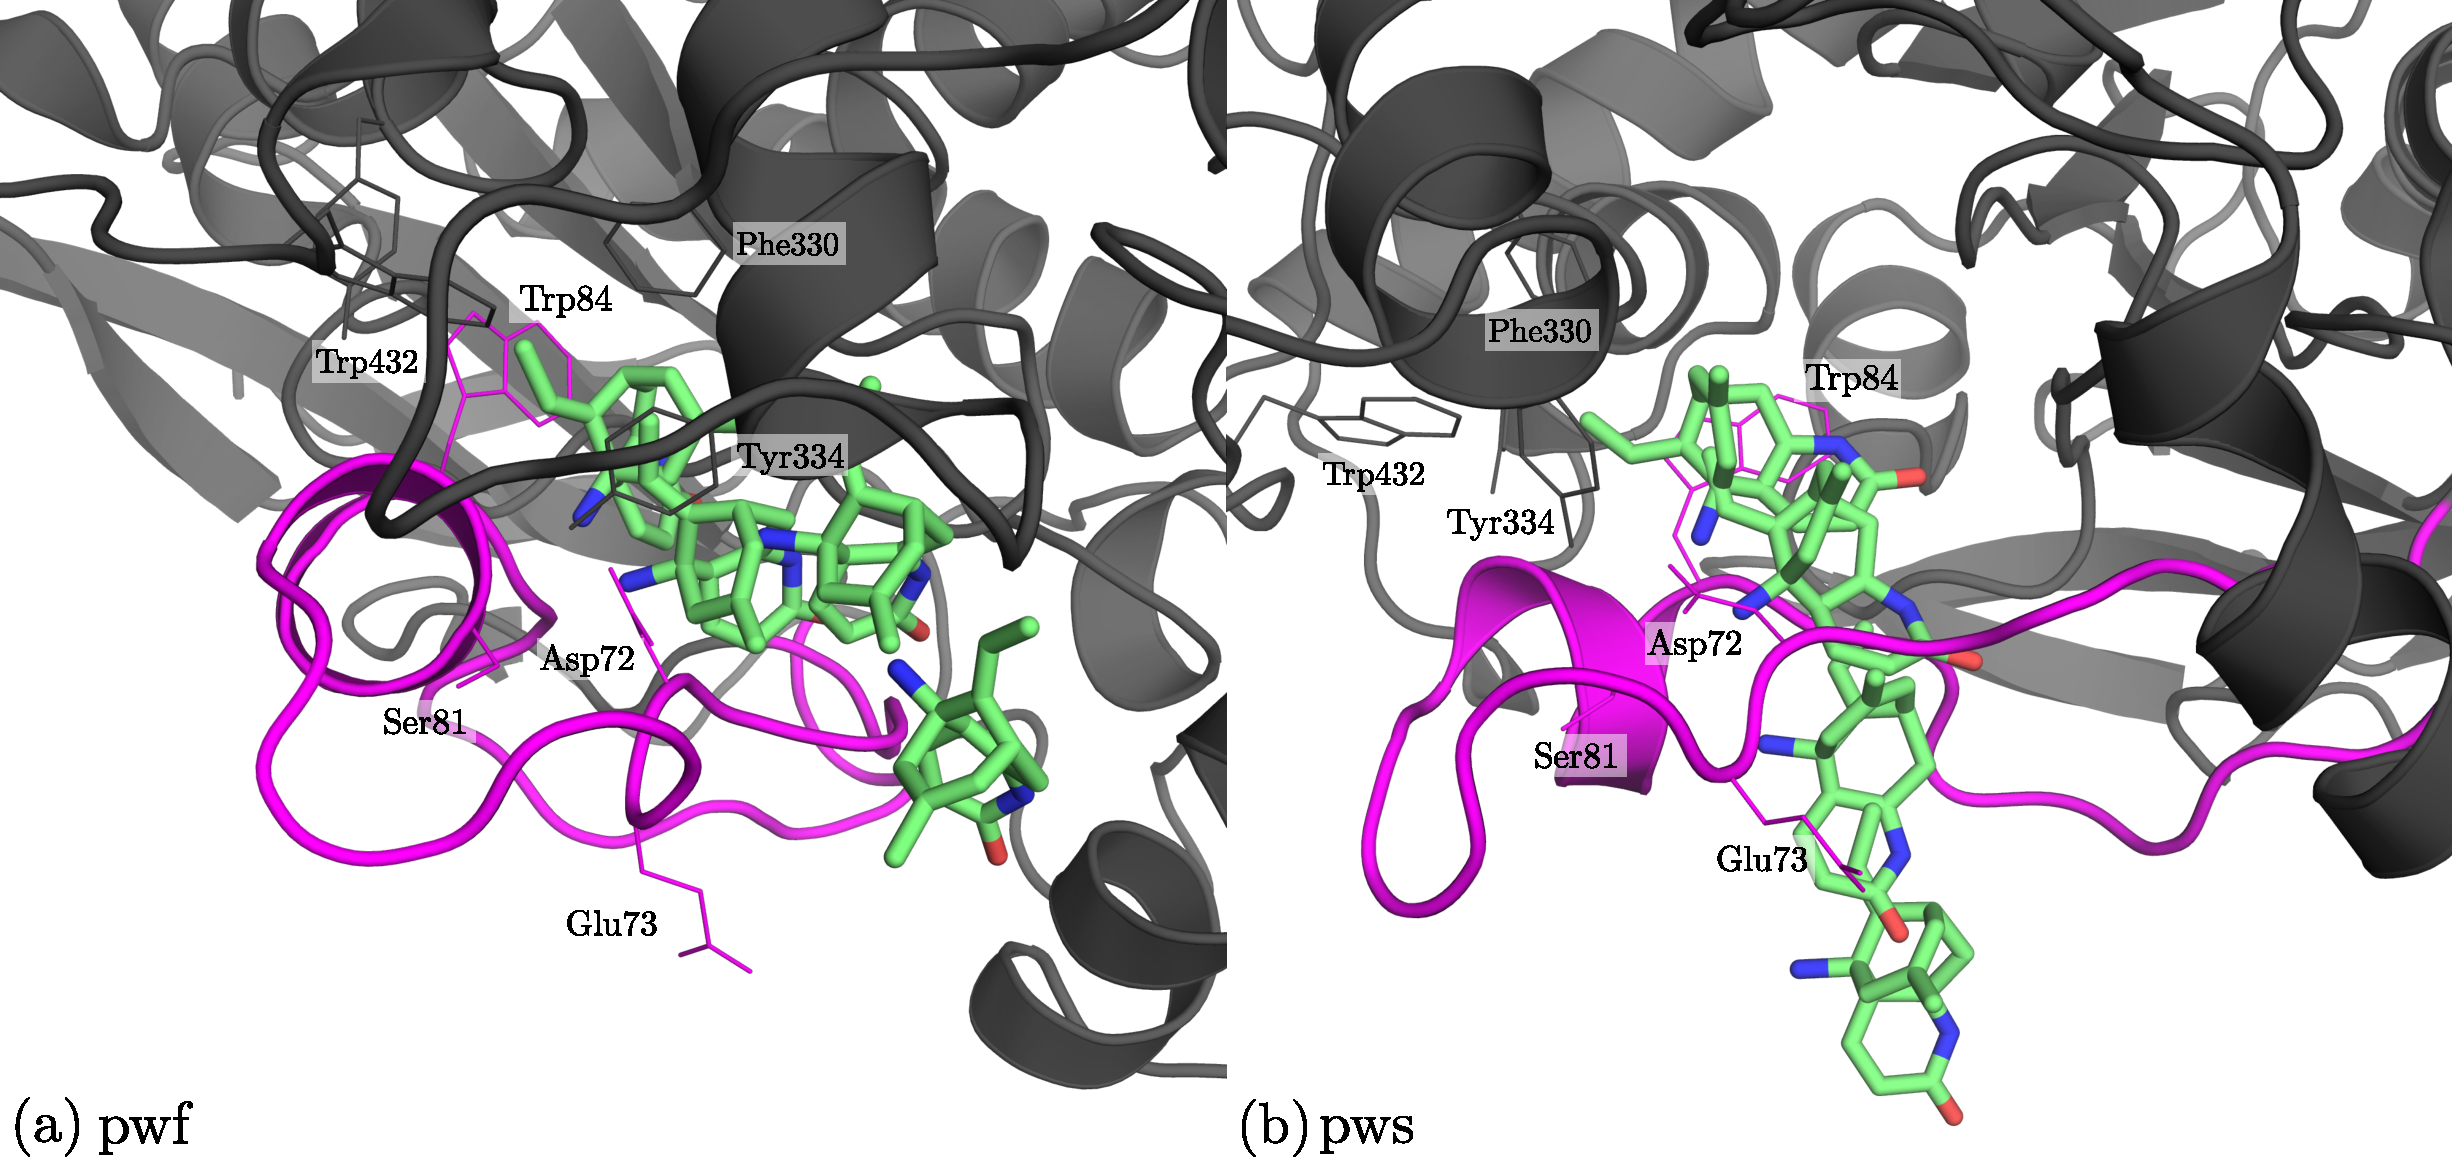
\includegraphics[width=38cm]{../fig/fig_6.pdf}
\end{minipage}

\noindent Structural representation of intermediate unbinding configurations along the RPs
which atomistically characterize the dissociation of hupA (shown as sticks)
along (a) pwf and (b) pws.  (pwf) or through the partially disorderedΩ-loop

\begin{minipage}[b]{0.5\linewidth}
  \centering
  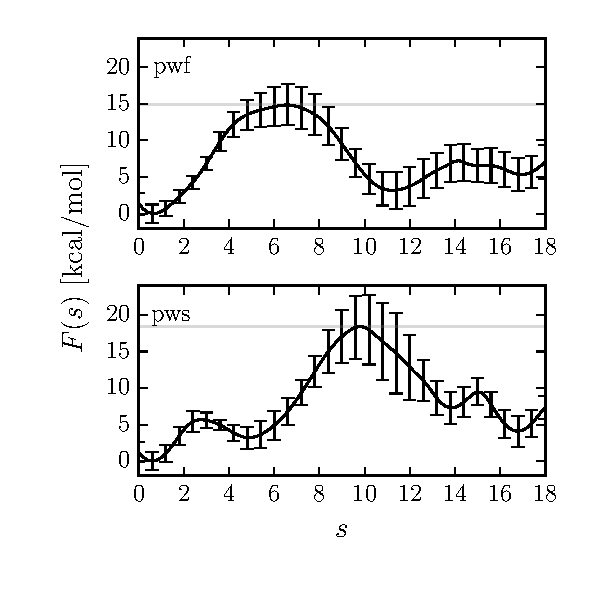
\includegraphics[width=20cm]{../fig/fig_7.pdf}
\end{minipage}
\hspace*{1cm}
\begin{minipage}[b]{0.4\linewidth}
  \begin{itemize}
    \bi Free-energy profiles along hupA dissociation pathways pwf and pws;
    \bi The error bars are calculated as standard errors from the well-tempered
      metadynamics simulations.
  \end{itemize}
  \vspace*{6cm}
\end{minipage}

\section*{\huge\centering\color{myblue}Are Transient Pathways Heterogeneous?}
\vspace*{1cm}
\begin{minipage}[b]{\linewidth}
  \centering
  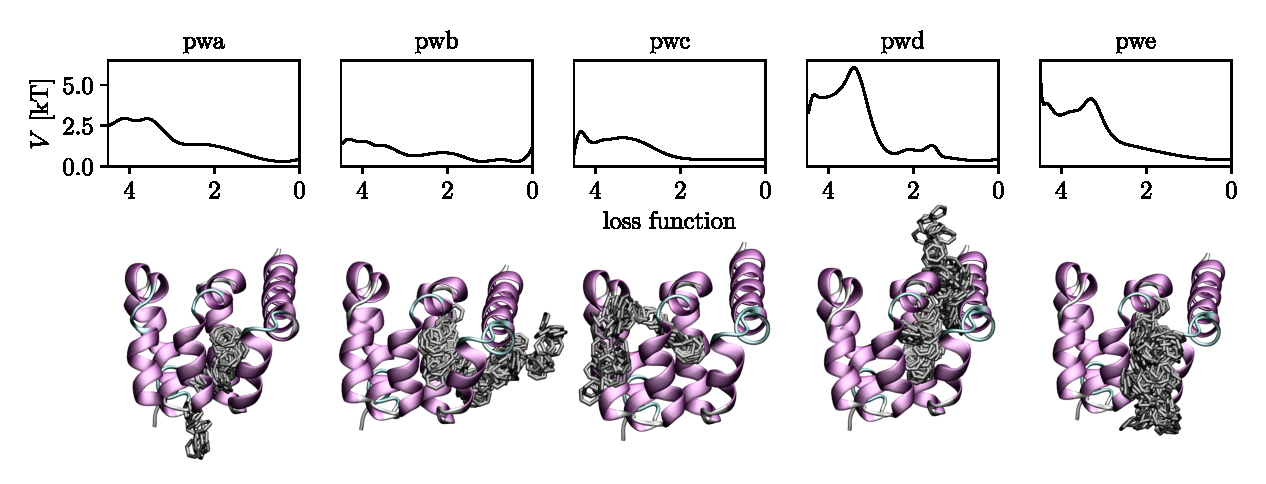
\includegraphics[width=36cm]{../fig/figx.pdf}
\end{minipage}

\noindent Reaction pathways of the benzene unbinding from the lysozyme L99A mutant
classified infive clusters.  In the upper panel the bias potential is shown as
a function of the minimized loss function.  The bottom panel depicts
atomistically the reaction pathways.

\section*{\huge\centering\color{myblue}\texttt{maze}: A Module for Plumed 2}
\vspace*{1cm}
\begin{minipage}[b]{\linewidth}
  \centering
  
\includegraphics[width=20cm]{../fig/maze-icon.png}
\end{minipage}
\vspace*{1cm}

\noindent\texttt{maze} is a code that implements enhanced sampling methods for simulating 
the reaction pathways of ligand unbinding. It is made as a module for Plumed 2, an
engine for free energy calculations of atomistic systems.
\vspace*{1cm}

\begin{minipage}[b]{0.5\linewidth}
  \centering
  
\includegraphics[width=12cm]{../fig/github.png}\\[1cm]
  \large Fork \texttt{maze} from Github.
\end{minipage}
\begin{minipage}[b]{0.5\linewidth}
  \centering
  
\includegraphics[width=12cm]{../fig/gitter.png}\\[1cm]
  \large Ask us on Gitter.
\end{minipage}

\color{myblue}
\begin{thebibliography}{6}%
\color{black}
\bibitem{1} J. Rydzewski, \dots, H. Grubm\"{u}ller. \textit{J. Chem. Theory Comput.} 14, 2843 (2018).
\bibitem{2} J. Rydzewski, O. Valsson, \textit{J. Chem. Phys.} 150 (2019).
\bibitem{3} J. Rydzewski, \textit{Submitted} (2019).
\end{thebibliography}
\color{black}

\section*{\color{myblue} Contact}
\begin{itemize}
    \bi Jakub Rydzewski \texttt{jr@fizyka.umk.pl}
\end{itemize}

\section*{\color{myblue} Acknowledgments}
We thank R. Jakubowski, W. Nowak, and M. Parrinello for useful discussions.
This work is supported by the National Science Centre, Poland (grants
2016/20/T/ST3/00488 and 2016/23/B/ST4/01770). The MD simulations were computed
using facilities of Interdisciplinary Centre of Modern Technologies, Nicolaus
Copernicus University, Poland.
\\
\\
All the data and PLUMED input files required to reproduce the results reported in
this study will be available on PLUMED-NEST (\texttt{www.plumed-nest.org}), the public
repository of the PLUMED consortium. 

\end{multicols}
\end{document}
